%%%%%%%%%%%%%%%%%%%%%%%%%%%%%%%%%%%%%%%%%%%%%%%%%%%%%%%%%%%%%%%%%%% 
%                                                                 %
%                            CHAPTER                              %
%                                                                 %
%%%%%%%%%%%%%%%%%%%%%%%%%%%%%%%%%%%%%%%%%%%%%%%%%%%%%%%%%%%%%%%%%%% 

\chapter{Literatuurstudie}

\section{Indoor navigatie \& visie}
        Op visie gebaseerde navigatie is een onderwerp dat zeer vaak onderzocht wordt.
        
    \section{Object detection}

        Een belangrijk aspect van dit onderzoek is het detecteren van individuele objecten in het beeld van 1 enkele RGB camera.
        De te detecteren objecten zijn op voorhand vastgelegd, en zijn afhangkelijk van de ruimte waarin de robot zich bevindt.

        In de logistieke gangen van een ziekenhuis zijn er heel wat objecten te zien die we kunnen detecteren, een kleine selectie van deze objecten zijn.

        \begin{itemize}
            \item Pictogrammen
            \item Brandblussers
            \item Deurklinken
        \end{itemize}

        Voor deze objecten gaan we kijken naar detectie technieken uit de traditionele beeldverwerking, en naar meer \textit{state of the art} technieken. 


        \subsection{Traditionele object detectie}
            In openbare gebouwen zijn er heel wat pictogrammen te vinden zoals nooduitgang, hoogspanning en brandblusser. Deze pictogrammen hebben steeds een specifieke vorm, kleur en symbool.
            De literatuur leert ons weinig over pictogramdetectie, maar pictogrammen kunnen wel vergeleken worden met verkeersborden die bijna dezelfde kenmerken hebben.
            De aanpak van~\cite{Fang2003} is om 2 soorten features in een beeld te onderscheiden. In eerste instantie detecteren ze vormen op basis van kleur randen en anderzijds wordt de
            afbeelding omgezet naar HSI waaruit enkel de hue gebruikt wordt. De hue is de belangrijkste component voor het onderscheiden van kleuren omdat er zo geen rekening wordt gehouden
            met de hoeveelheid licht en schaduwen.
            Een recenter onderzoek~\cite{Zabihi2017} bouwt voort op deze technieken,
            maar bereken de Histogram of Oriented Gradients (HOG) features van het beeld. Vervolgens wordt er gebruik gemaakt van een Support Vector Machine (SVM) om te bepalen waar er zich een match bevindt.

            Vervolgens kunnen de vorm en kleur features gecombineerd worden om de plaats voor een mogelijke match te vinden. Eens er een mogelijke boundig box gevonden is,
            kan er geprobeerd worden een template te matchen om het effectieve pictogram te achterhalen. Het grootste probleem bij de techniek van~\cite{Fang2003} is
            dat hun gebruikte template matching techniek niet robuust is voor schaal invarianties.
            Bij~\cite{Zabihi2017} maken ze voor de herkenningsfase gebruik van SIFT\cite{Lowe1999} features en kleur informatie. 
            Hierbij worden de SIFT features van de kandidaat matches en de templates vergeleken, en er wordt een gemiddelde genomen van de verschillen tussen hue, saturation en value.
            Door middel van RANSAC en een treshold wordt er bepaald welke matches gebruikt worden.

        
        \subsection{Convolutional neural nework}
            Een convolutional neural network of CNN is een supervised deep learning techniek die gebruikt kan worden om complexere beeldinterpretatie te doen.
            Een CNN kan bestaan uit meerdere lagen die meestal een combinatie zijn van 'convolutional-layers' en 'fully connected-layers'. Elk van deze lagen bevat een aantal neuronen met elk een eigen set van gewichten.
            Het doel van een CNN is om de gewichten zodanig bij te stellen zodat data die aan de eerste laag gegeven wordt een verwacht resultaat geeft aan de laatste laag. 
            Deze laatste laag kan men de classificatielaag noemen, en geeft een representatie van wat het netwerk denkt dat er aan de input staat. In figuur~\ref{fig:yolo_cnn} is een voorbeeld tezien van een CNN met de verschillende soorten lagen.

            \begin{figure}[!hb]
                \centering
                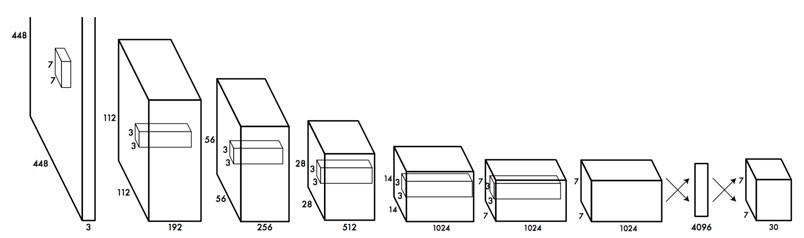
\includegraphics[width=0.75\linewidth]{yolo_cnn.jpeg}
                \caption{De lagen van een CNN volgens het YOLO~\cite{Redmon_2016} detection system.}
                \label{fig:yolo_cnn}
            \end{figure}

            Een 'convolutional-layer' is een laag die een convolutie operatie uitvoert op zijn input, het resultaat van deze operatie is een kleinere dataset die gebruikt wordt als input voor de volgende laag.
            De convolutie kan toegepast worden op meerdere dimensies in 1 keer waardoor de output een tensor zal worden.

            Om een CNN te gebruiken, dient het 'getraint' te worden. Voor de training van een netwerk zijn er 2 dingen noodzakelijk, veel voorbeeld data en per voorbeeld de verwachte output.
            De loss functie is een maat van hoe goed een netwerk een voorspelling kan doen van de input data, met andere woorden een vergelijking tussen de input en de output. Het doel van de training van een netwerk is het minimaliserem
            van deze loss functie. Dit kan gedaan worden d.m.v 'backprogagation'. Backpropagation is het steeds een klein beetje aanpassen van de gewichten in de inwendige neuronen om zo het resultaat te verbeteren en de loss functie te verkleinen.
            Een netwerk heeft een goede training gehad als de loss functie minimaal is.
            

    \section{Object tracking}

    \section{Image segmentation}
        Het correct segmenteren van de beelden zal een belangrijke rol spelen. Niet in elk beeld zal er een destinctief object aanwezig zijn om te detecteren. Daarom is het belangrijk om de vloer van
        de muren te kunnen onderscheiden. Een eenvoudige approach zou kunnen zijn om via K-means een verdeling van een beeld te doen en met een soort regressie de regio's te labelen. 
        Volgens~\cite{zhangwall} werkt de K-means aanpak met een op textuur en kleur gebaseerde aanpak redelijk goed, maar wordt steeds de muur verbonden met het plafont omwille van kleur en textuur gelijkenissen.
        Hun regressie gebaseerde labeling techniek blijkt echter een slechte oplossing. Verder zoals~\cite{Li2010} aangeeft zijn reflecties en overbelichting eigenschappen van indoor omgevingen die het moeilijk kunnen maken om
        een correcte segmentatie te doen.